% CRIPTOMOEDAS
\subsection{\textbf{O que são criptomoedas?}}

Por definição, criptomoedas são qualquer tipo de moeda digital ou virtual que utiliza criptografia para garantir a realização de transações. Elas não têm autoridade central de emissão e nem regulação. Em contrapartida, elas utilizam um sistema de criptografia chamado de blockchain, além de outros sistemas de criptografia descentralizados para registrar transações e emitir novas unidades. 

\textbf{Blockchain é um banco de dados distribuído que consegue fazer um} compartilhamento de informações dentro de uma rede. Essas informações podem ser variadas, agrupadas em bloco a partir de criptografia, de uma forma que consiga trazer consigo o histórico completo e imutável das transações anteriores. Assim, garantindo uma rede de operações concisas, seguras e confiáveis para qualquer um que desejar participar dessa rede.

As criptomoedas atuam com diversas funções e objetivos além de um simples meio de transação monetária para uso diário. Elas podem servir como reserva de valor; atuar como \textbf{ativos de investimento}, devido à sua alta volatilidade; descontos em taxas; garantia de algum serviço; entre muitas outras funções.

Um dos maiores exemplos de criptomoedas são o Bitcoin e o Ether. O \textit{Ether} valendo cerca de \textbf{2.650 dólares americanos}, além do \textit{Bitcoin}, ultrapassando mais de \textbf{108 mil dólares americanos} e sendo a criptomoeda mais famosa do mundo. (Valores retirados no dia 16/06/2025)
% BITCOIN
\subsection{\textbf{O que é \textit{Bitcoin}?}}

Lançado em 2008, com o pseudônimo de \textit{Satoshi Nakamoto}, uma nova ideia foi criada e posta ao mundo, com a criação do \textbf{Bitcoin}. O Bitcoin é atualmente a criptomoeda mais famosa do mundo, além de ser a mais valorizada atualmente, ultrapassando a marca de US\$100.000,00 e chagando a valores superiores.

Por ser uma criptomoeda, o Bitcoin não possui uma emissão regularizada e centralizada, a emissão de novas moedas no mercado é de uma outra forma. É usado o termo "mineração". Esse processo consiste na resolução de quebra-cabeças matemáticos complexos feitos por hardware e software especializados para a mineração de Bitcoin. A mineração não é exclusiva de um grupo de pessoas, empresas ou bancos. Desde que tenha energia e um hardware de mineração, é possível obter um bloco de Bitcoin.

Os blocos de Bitcoin são os produtos e agrupamentos de transações individuais dos últimos dez minutos de cada mineração. Cada bloco é único e fechado, cada um criando seu próprio número \textit{Hash}, que é onde estão codificadas as transações. Cada novo bloco precisa ter em seu conteúdo as informações do bloco anterior, o que garante uma veracidade de que não será manipulado ou alterado. Cada bloco gerado é equivalente a uma quantidade específica de Bitcoin, cada bloco tem atualmente 3.125 BTC (Bitcoin).

Essa unicidade garante que cada unidade da moeda não possa ser possuída por mais de um portador. O que torna a concorrência de cada máquina para garantir seu bloco próprio maior ainda, incentivando cada vez mais a melhora dos computadores para fazer a mineração. Além disso, para a autenticação no sistema de Prova de Trabalho (PoW) do Bitcoin, os computadores de mineração precisam comprovar a energia gasta para a mineração de cada bloco. Isso reforça a segurança e autenticidade de cada máquina e bloco minerado.

% Gráfico Principal
\begin{figure}
    \centering
    \shadowbox{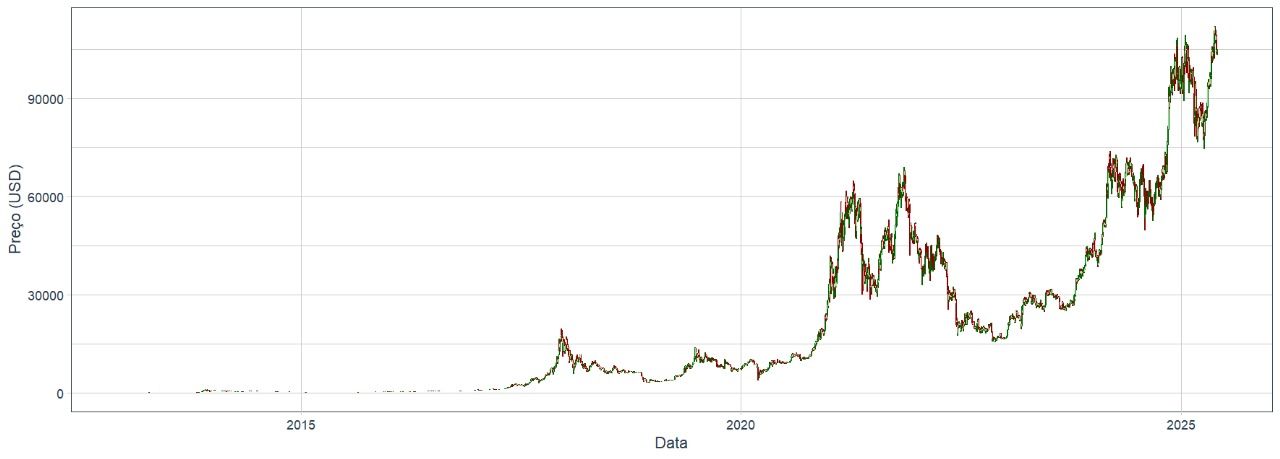
\includegraphics[width=1\linewidth]{Imagens/Grafico-Princial.jpg}}
    \caption{Histórico do Valor do Bitcoin}
    \label{fig:Candle Graph}
\end{figure}

% EVENTOS IMPORTANTES
\subsection{\textbf{Eventos Importantes:}}

A Lei da Oferta e Demanda tem grande influencia sobre a valorização e  desvalorização do Bitcoin.  Assim como nos mercados tradicionais, quando a oferta de um produto é limitada e sua demanda aumenta, o seu valor tende a aumentar também. Só que no caso do Bitcoin, ele é tanto o produto quanto uma possível moeda de troca externa. Isso tudo é realçado por ter uma oferta limitada à no máximo 21 milhões de unidades. No entanto, também existem outros fatores que podem influenciar  em seu valor, tendo os principais exemplos ocorridos: o evento Halving; a queda da Mt. Gox e a pandemia de COVID-19.

Ocorrendo aproximadamente a cada 4 anos, o evento Halving  reduz pela metade o ganho de Bitcoin por bloco minerado, diminuindo a entrada de novos bitcoins no mercado. Este evento é associado geralmente com a valorização do bitcoin, já que aumenta a escassez da moeda, favorecendo a sua valorização.

Acontecimentos externos também podem ocasionar a desvalorização da moeda, como por exemplo a falência da empresa Mt. Gox, em 2014. Na época, a maior corretora de criptomoedas do mundo, acabou perdendo por volta de 800 mil bitcoins após sofrer uma sequência de invasões cibernéticas. Isso causou uma queda brusca no valor do bitcoin e afetando a confiança neste mercado.

A pandemia de COVID-19 em 2020 também teve um grande impacto no valor do bitcoin. Com a incerteza global ao início da pandemia, o Bitcoin apresentou uma queda em seu valor, porém com a desvalorização das moedas fiduciárias, o Bitcoin passou a ser procurada como investimento alternativo, resultando em uma significativa valorização.